\documentclass[a4paper]{report}
\usepackage[margin=0.5in]{geometry}
\usepackage{longtable}
\usepackage{listings}
\usepackage{graphicx}
\usepackage{multirow}
\usepackage{fontspec}
\usepackage[section]{placeins}


\title{Lab8\_Kogge Stone Adder design}
\author{201704150 Kangjun Heo}

\lstset{basicstyle=\ttfamily,breaklines=true}
\lstset{framextopmargin=10pt,framexbottommargin=10pt,frame=tb}


\begin{document}
    \maketitle
    \tableofcontents

    \chapter{Purpose of the lab}

        \paragraph{This lab aims to design 16bit Kogge Stone Adder with Verilog language. This report contains state diagrams, waveforms and verilog codes with test cases.}
    
        \section{Kogge Stone Adder}

        \paragraph{\normalfont Kogge Stone Adder is a sort of Carry Propagation Adder(CPA), generates carry output and sum with parallel carry look-ahead tree. It implements 'dot', which achieves associativity that enables to parallelize carry operations.}

        \paragraph{\normalfont In this lab, 16 bit Kogge Stone Adder will be implmeneted, which gets 2 16-bit sized inputs and carry-in, outputs 1 16-bit sized data and a bit of carry out.}
        

    \chapter{Design Procedure}
        \begin{figure}[!htb]
            \centering
            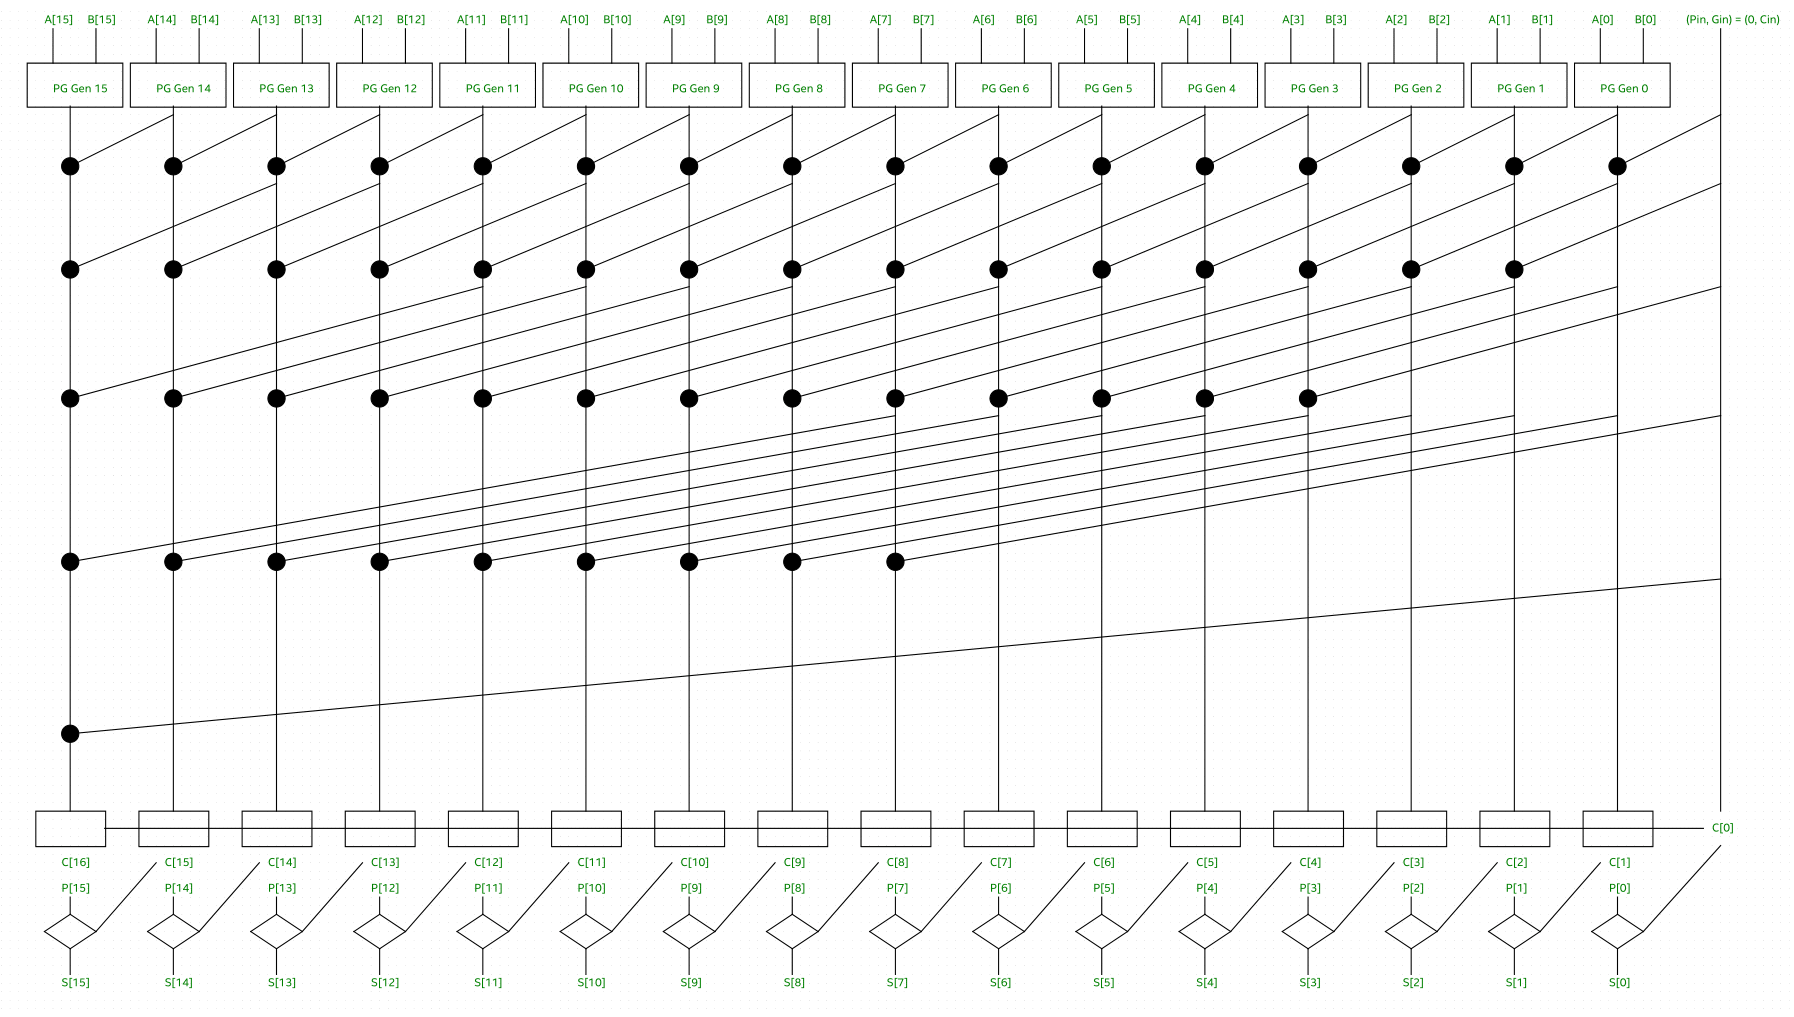
\includegraphics[width=\textwidth]{diagrams/ksa_16b-1.png}
            \caption {Block diagram of the desired Kogge Stone Adder}
            \label{fig:wf-0}
        \end{figure}
        

    \chapter{Simulation}
        \section{Source Code}
            \lstinputlisting[caption=Top Module of Kogge Stone Adder]{ksa_16b/ksa_16b_top.v}
        \section{Testbench}
            \lstinputlisting[caption=Testbench Code]{ksa_16b/ksa_16b_tb.v}

        \section{Simulation Result}
            \begin{figure}[!htb]
                \centering
                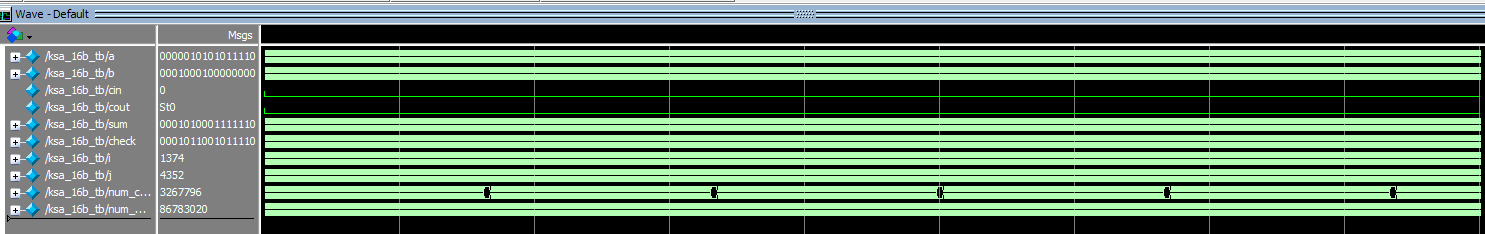
\includegraphics[width=\textwidth]{diagrams/long_test_result.PNG}
                \caption {Waveform of Long Test}
                \label{fig:wf-1}
            \end{figure}

            \begin{figure}[!htb]
                \centering
                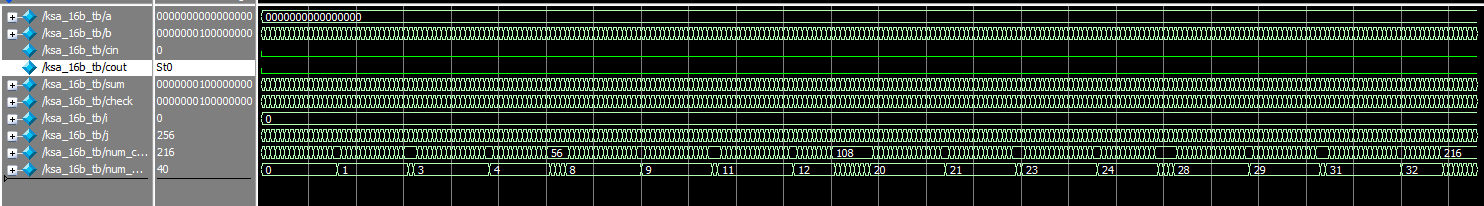
\includegraphics[width=\textwidth]{diagrams/short_test_result.PNG}
                \caption {Waveform of Short Test (256 cases)}
                \label{fig:wf-2}
            \end{figure}

            \begin{figure}[!htb]
                \centering
                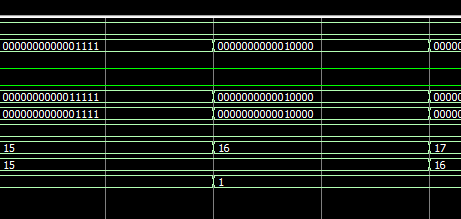
\includegraphics[width=\textwidth]{diagrams/waveform_bug.PNG}
                \caption {Detected Testing Glitch}
                \label{fig:wf-3}
            \end{figure}

    \chapter{Evaluation}
        \paragraph{\normalfont For precise testing, $65535 \times 65535$ (4294836225) cases of testing were going to be executed - for each inputs, (0000000000000000 to 1111111111111111, about 43 seconds in modelsim time - however, too much time was taken therefore 900508160ns(about 9 seconds in modelsim time) of test were actually executed. and the result was same as below:}

        \begin{itemize}
            \item Correct Result: 3267796
            \item Wrong Result: 86783020
        \end{itemize}

        \paragraph{\normalfont Also, additional test were conducted for 2560 nanoseconds for validating 4bit inputs: }

        \begin{itemize}
            \item Correct Result: 216
            \item Wrong Result: 40
        \end{itemize}

        \paragraph{\normalfont This can be considered as some kind of timing issue or glitch of ModelSim (it can't be though) - or there's unknown problem that I couldn't find.}

    \chapter{Discussions}
        \section{Key Part of This Lab}
            \paragraph{\normalfont There were 5 stages of Carry Look-Ahead tree, which has decreasing black cell operation for each stage, with regular count. each (P, G) pair is combined with previous inputs.}

        \section{Mistakes}
            \paragraph{\normalfont Because of the characteristics of KSA logic circuit, Organizing each CLA tree stage caused several glitches and compilation errors. There's a rule that combining for each term P and G, it is important to understand strictly about it. }

        \section{Expected Improvements}
            \paragraph{\normalfont Conditional branches are useful when designing modules in behavior form. However, Its mechanism is not exactly same as other C-like languages so different plotting is required when using it.}
\end{document}